\documentclass[12pt]{article}
\usepackage{lingmacros}
\usepackage{tree-dvips}
\usepackage{datetime}
\usepackage{color}
\usepackage{graphicx}
\usepackage{cite}
\graphicspath{ {images/} }
\title{Master thesis proposal}
\author{Ion Madrazo Azpiazu}
\date{\today}
\begin{document}


\maketitle
\section{Introduction}

Reading is an important skill in the academic environment, a skill that can be deciding for a student's educational opportunities and their career \cite{robinson2000issues}. Therefore, giving students students encouraging texts to read during each of the stages of their lives is essential. Even outside the educational environment, reading plays a important role. It is primordial for people that get good understanding from the texts they read, specially when they face medical or legal issues. Understanding a legal or medical document properly, can lead the reader to taking a better decision and having more confidence about  it. However, studies\cite{medicalReadability1}\cite{medicalReadability2}\cite{medicalReadability3} show that even medical resources that are supposed to be suited for average readers, tend to be too specialized and even well educated adults have trouble understanding. Being able to produce simple texts, that can be understood by people with low reading skills seems imperative.\\



A readability score refers to the degree of ease with which a reader can understand a given text and score which is usually determined by a readability formula. Historically, teachers have been the main stakeholders of the use of readability formulas, making use of them for obtaining new materials for their courses and curriculum design. However, lately, readability scores have been discovered to have more uses than the ones in academic environments. Automatic text simplification\cite{textsimplification1}\cite{textsimplification2} or summarizing for people with reading difficulties\cite{textsimplificationWithDisabilities1}, book recommendation \cite{pera2014automating}, literacy assessment\cite{literacy1}, or even legal\cite{legalreadability} and medical document complexity assessment\cite{medicalReadability1}\cite{medicalReadability2}\cite{medicalReadability3} are only a few examples of the benefits a readability score can provide.\\


During a few decades, traditional formulas such as Flesh \cite{flesch1948new}, Dale-Chall \cite{chall1995readability} and Gunning FOG  \cite{albright1996readability} became very popular among the educators for manually determining text difficulty. Most of those formulas made use of \textit{shallow features} such as, average word length or average sentence length, which provided a simple way of determining a texts complexity, despite lacking precision in some cases. Cases such as the one claimed by (David and kantor 1982){\color{red}(manually cited)} where nonsense text could be classified as simple to read, just because it contained short and frequently used words. Cases like that  encouraged researchers to study better methods of prediction.   Therefore, over time, the traditional shallow formulas started to leave place to more complex formulas\cite{franccois2012ai}\cite{aluisio2010readability}, that began to put together both natural language processing and machine learning techniques. The new formulas usually continued using the shallow  features  mentioned above, but added new more complex features based on syntax or semantics of the text. With the addition of new features, the tools became more precise, but more constrained regarding the language. They started to use more and more language dependent techniques and tools, which made the systems difficult to adapt to other languages than the one they were designed for, making the multilingualism that was possible in the early stages disappear.  \\


Having seen the lack of multilingualism among the state of the art systems for readability prediction, we propose to develop a multilingual readability assessment tool . This tool should both show results comparable to monolingual state of the art systems,  and  maintain the multilingualism the early tools in the readability field had. For doing so we will make a exploration of the features and methods used in literature, and adapt them to be multilingual. Furthermore, we will develop novel features  and that will aim at being useful for each of the languages, individually or collectively. Finally, we will analyze the effect each of the tested features have regarding readability, determining by this, what features make a text readable generally and specifically for each language. In doing so, we will produce a system that will adapt itself to the input text language, and use an adequate subset of features for that certain language for giving a prediction, creating, to the best of our knowledge, the first multilingual readability assessment system.\\


It is important to note, that for practical purposes, the application will only be tested in three different languages: \textit{English}, for state of the art comparison purposes and as reference of germanic languages. \textit{Spanish}, as a reference for latin languages, and \textit{Basque} as an example of a non-indoeuropean language.



\section{Thesis statement}
{\color{red}Let's discuss about this section next meeting, looks like a big repetition of paragraph 4 to me.}\\

 We aim to develop a multilingual readability predictor taking advantage of machine learning techniques and features extracted using natural language processing techniques. As a secondary goal, we will survey the features and methods currently used in the state of the art, and create a comparison features and their importance in the readability prediction for each language. As a byproduct of the development and testing, we will create various datasets that can be of good use for other researchers in the area.


\section{Related work}
In the recent years, different Readability Assessment (RA) systems have been developed with high diversity regarding both languages and features. \\

{\color{red} I have spent some time looking for multilingual tools and it looks that there is nothing. Where should I talk about that?  Maybe in previous paragraph? Or right at the end of the RW? } \\



For \textbf{English}, \cite{feng2010comparison} presented a comparison of the common readability features used for English. \cite{aluisio2010readability} aimed their system for evaluating text simplification methods with a system, that made use of some more elaborated features such as ambiguity in terms. \cite{feng2009automatic} oriented their system for assessing the difficulty level of a text for people with intellectual disabilities, developing some features that were intended to detect how well a text was structured. {\color{red} Will find a couple more.} \\  

For \textbf{Spanish} several systems\cite{vstajner2013readability}\cite{drndarevic2013automatic} have focused their work on text simplification and its evaluation using classical readability formulas. Formulas such as, SSR \cite{spaulding1956spanish} based on sentence length and number of rare words per sentences or LC and SCI \cite{anula2007tipos} based on density of low frequency words in text. {\color{red} Let's try to find another one. Not so easy here.} \\


For \textbf{Basque}, for the best of our knowledge, only one system have been developed. Due to the fact that Basque is considered a minority language and shares very little similarities with the most spoken languages. Very little research have been done in the area. Therefore, currently, Errexail \cite{gonzalez2014simple} is the only system created for Basque readability assessment. This system was aimed for text simplification purposes and was developed to predict two different values, simple or complex. The aim for this was to detect which texts needed some simplification and which texts did not. The system makes use of simple features mostly based on ratios of common Natural language processing tags.\\



For \textbf{Chinese}, \cite{chen2011chinese} developed a RA system only based on lexical metrics based on the TF-Idf measure. This metric in conjunction with a mutual information measure was able to determine which terms were most relevant for each of the readability levels. These terms were afterwards used to predict the level of readability for the inputs texts. However, this technique was not topic independent, as once trained for a certain topic the terms were no longer useful for other topics. Previously, \cite{collins2004language} developed a system that already tried to solve, the topic dependence problem for Chinese. This system was based on Tf-Idf too and as the authors stated, removing some top scoring words of the Tf-Idf ranking, lead the system to be more independent of the topic. Apparently, the top scoring words were highly specialized words to the topic selected for training.\\

For \textbf{Arabic}, \cite{al2008towards} developed a readability assessment told based on only two features. The features were based on simple ratios based on sentence,terms and letter counts. Those, features were used with a SVM classifier in order to be able to classify text as simple or complex.\\

For \textbf{Italian}, \cite{dell2011read} presented a readability assessment system aimed for text simplification. Since the text simplification tool the authors were developing was based on sentences. The authors of this system decided,that rather than developing a system for determining text readability, their system would work at sentence level. Therefore, the text simplification tool, would have more information of which sentence needed simplification and which did not. The model generated for sentence level is shown to be generalizable to full text level, by the use of simple averages. The more complex sentences a text have, the more probabilities it have to be complex in overall.\\

For \textbf{French},\cite{franccois2012ai} developed a readability assessment system with the foreign language learners in mind. The objective was to determine which features were more important for a foreign language learner to understand a text. In addition, they provided a metric new to the area called adjacent accuracy that tried to measure systems' performance in a more accurate and relevant. \\



\section{Methodology}
The proposed method relies in two different areas of data science, Natural language processing and machine learning. Advantage of one or both areas is taken in each of the steps that conform the pipeline of the algorithm explained below.
\subsection{Pipeline description}
The pipeline of the algorithm if composed by the following steps: Texts processing, feature extraction, feature processing and prediction. A visual description of the general pipeline of the system can be seen on figure \ref{fig:pipeline}.  A more in-depth explanation of each step can be seen in the following sections.

\begin{figure}[h]
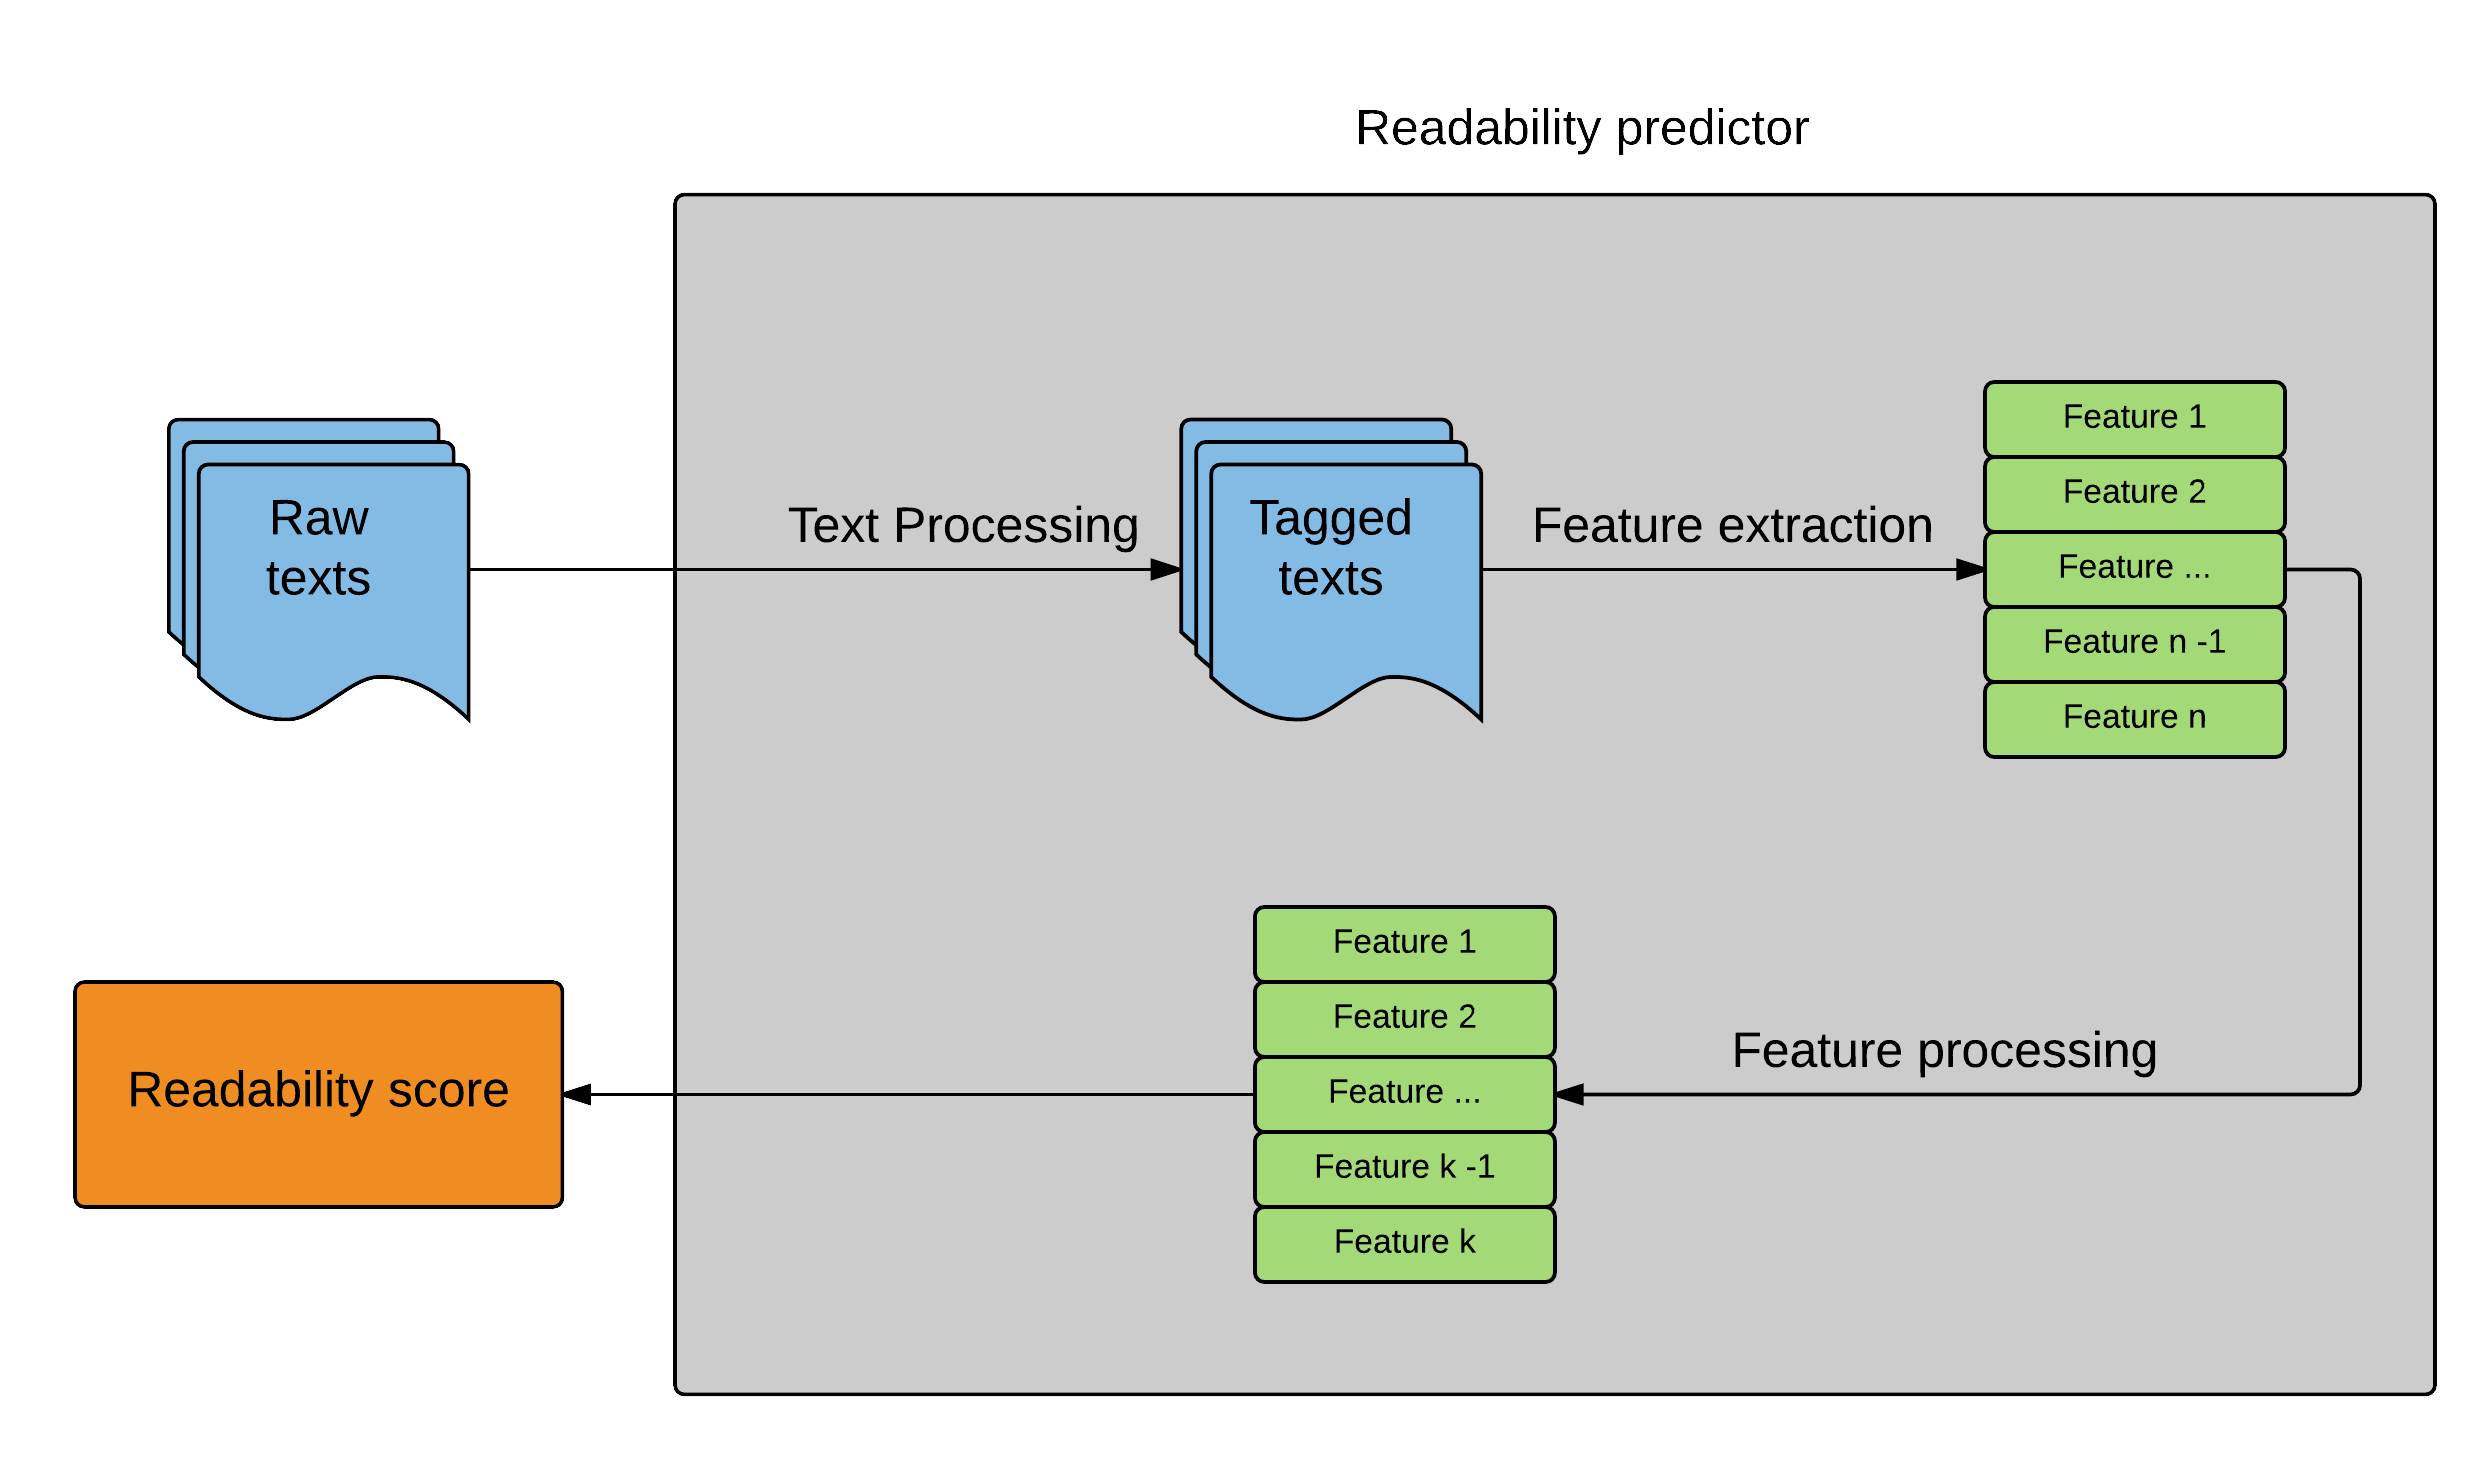
\includegraphics[width=\textwidth]{pipeline}
\caption{General pipeline}
\label{fig:pipeline}
\end{figure}

\subsection{Text processing}

The text processing step is the step where the raw text is given structure and, therefore, value. This structure and information will later be used for extraction features that will help the system predict a readability score.\\

The tool that has been chosen for natural language processing is Freeling NLP\cite{freelingNLP}. Freeling is an open source Natural language processing library that supports 11 different languages. The tool solves common NLP tasks, such as, Tokenization, sentence detection, Part of speech tagging or dependency parsing. Each of this processes will be helpful for building certain features later.\\

The \textbf{tokenization} is the base module for any NLP processing. Tokenization refers to taking a raw text and normalizing it into pieces that make text processing possible. This will also make possible, to implement tradition shallow features such as, Flesch–Kincaid \cite{flesch}. \\

The \textbf{Part of speech} analysis determines the function each token has in the sentence. This, together with \textbf{dependency parsing} techniques, make possible the analysis of syntactic structures in the sentences.\\

Other tools outside Freeling, such as \textbf{WordNet} or \textbf{Latent semantic analysis} techniques, will make possible to analyses texts at semantic level, for detecting structures that refer to concepts rather than to tokens themselves.\\


\subsection{Feature extraction}
This section describes the features proposed for the system. These features range from the most simple and commonly used ones such as the shallow features, to a more complex set of features such as the ones base on semantics.

\subsubsection*{Shallow features}
\subsubsection*{Part of Speech tags}

\subsubsection*{N-grams}

...

Description of all the features used. Why should this feature be valuable, give hypotheses and intuition behind the use of each feature. Give examples when needed.

\subsection{Feature processing and selection}
Describe algorithms used for feature processing and selection, why should they help get better results?

\subsection{Learning and prediction}
Describe algorithms for learning and prediction. Pros an cons of each algorithm, why should this algorithm adapt better to our problem?

\section{Evaluation}

\subsection{Datasets}
Information about how we get and extract the datasets.
\subsubsection{English}
\begin{itemize}
\item Lexile
\item List all for proposal...
\end{itemize}
\subsubsection{Spanish}
\begin{itemize}
\item Lexile
\item List all for proposal...
\end{itemize}
\subsubsection{Basque}
\begin{itemize}
\item Ikasbil
\end{itemize}

\subsection{Metrics}

\begin{itemize}
\item Error rate, accuracy
\item Adjacent accuracy, double adjacent accuracy...
\item Average error distance
\end{itemize}

\subsection{Tests}

\begin{itemize}

\item Which features add the most value? Correlation, information gain etc.

\item Do features correlate similarly with the readability score for each language?

\item Feature preprocessing, does it help?
	\begin{itemize}
	\item Discretization
	\item Feature subset selection techniques
	\end{itemize}
	
\item Comparison of learning models, which learning model fits best the problem?
	\begin{itemize}
	\item KNN
	\item Bayesian models
	\item SVM
	\item Neural network
	\item Regression (Adding a sense of order in class values)
	\item Ordinal classification (Adding a \textbf{stronger} sense of order in class values)
	\end{itemize}

\item \textbf{Comparison} of the system vs \textbf{baselines} such as fleish for each language individually.

\item Comparison \textbf{vs state of the art} systems for each language.

\item Multi vs monolingual
\item If we take a bilingual corpus, does the system predict same values? And if we take a text and translate it to another language? Does the readability values maintain using an automatic translator?
\end{itemize}



\bibliography{bibliography}{}
\bibliographystyle{apalike}
\end{document}